\documentclass[12pt]{extarticle}
\usepackage[utf8]{inputenc}
\usepackage[portuges]{babel}

\usepackage{lipsum} 
\usepackage{amssymb}
\usepackage{amsmath}
\usepackage{titling}

\usepackage{cite}

\usepackage{graphicx}
\usepackage{float}

\graphicspath{ {./Figures/} }

\title{Trabalho Prático 1\\
       \large{Arquitetura e Cálculo - 2019/2020}}
\author{Bruno Antunes - PG40866\\
        Pedro Moura - PG41094}
\date{\today}

\begin{document}

\maketitle


\begin{abstract}
	Modelação e análise de um sistema de tempo-real com base na ferramenta UPPAAL.
\end{abstract}


\tableofcontents

\newpage

\section{Introdução}
O presente relatório descreve o desenvolvimento do 1º trabalho prático da UC de Arquitetura e Cálculo, integrada no perfil de Métodos Formais em Engenharia de \textit{Software}, do 1º ano do Mestrado em Engenharia Informática da Universidade do Minho.

Este trabalho consiste na modelação e análise de um sistema de tempo-real através da ferramenta UPPAAL.

\paragraph{Enunciado}{\textit{
	In the middle of the night, four adventurers encounter a shabby rope-bridge spanning a deep ravine.
	For safety reasons, they decide that no more than 2 people should cross the bridge at the same
	time and that a flashlight needs to be carried by one of them in every crossing. They have only
	one flashlight. The 4 adventurers are not equally skilled: crossing the bridge takes them 1, 2, 5,
	and 10 minutes, respectively. A pair of adventurers crosses the bridge in an amount of time equal
	to that of the slowest of the two adventurers.
	One of the adventurers claims that they cannot be all on the other side in less than 19 minutes.
	One companion disagrees and claims that it can be done in 17 minutes.
}}

\paragraph{Objetivo}{
	Criar um modelo para este sistema e verificar, através de CTL, as seguintes propriedades:
	\begin{itemize}
		\item[-] é \underline{possível} que todos os aventureiros estejam do outro lado da ponte em 17 minutos;
		\item[-] é \underline{impossível} que todos os aventureiros estejam no outro lado da ponte em menos de 17 minutos.
	\end{itemize}
}

\newpage
\section{Modelação}
No sistema existem 3 tipos de autómatos: \textbf{Person} ($\times 4$), \textbf{Lantern} e \textbf{Bridge}.

Para além disso, é necessária a existência de algumas variáveis globais:
\begin{itemize}
	\item \texttt{L\_L} - inteiro que representa a localização da lanterna. $0$ se no início da ponte, $1$ se no fim;
	\item \texttt{L\_BUSY} - booleano que diz se a lanterna está ocupada ($true$), ou está livre ($false$). É inicializado a $false$.
	\item \texttt{global} - relógio global. 
\end{itemize}


\subsection{\textit{Lantern}}
\begin{figure}[H]
	\centering
	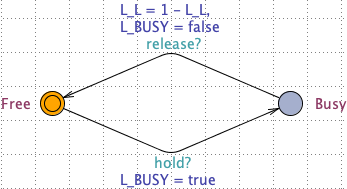
\includegraphics[width=10cm]{Lantern.png}
	\caption{\textbf{Lantern} - modelo.}
\end{figure}

O processo \textbf{Lantern} representa a lanterna.

Quando sincroniza através da ação \texttt{hold?}, significando que alguém pegou na lanterna, avança para um estado em que está ocupada, e a partir daqui, só com a transição \texttt{release?} é que volta a estar livre.
O modelo deste processo também faz com que seja impossível o sistema executar, por exemplo, 2 ações \texttt{hold!} seguidas, o que significa que apenas um aventureiro pode estar com a lanterna num certo momento.

De notar ainda que, como vamos ver a seguir, no fim de cada travessia, o aventureiro que possuir a lanterna tem de a libertar. Com isto, podemos atualizar a posição da lanterna aquando de um \texttt{release?}.


\subsection{\textit{Bridge}}
\begin{figure}[H]
	\centering
	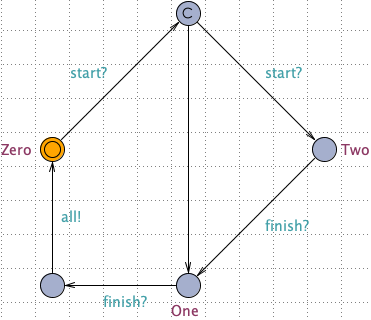
\includegraphics[width=10cm]{Bridge.png}
	\caption{\textbf{Bridge} - modelo.}
\end{figure}

O processo \textbf{Bridge} controla o número de elementos que realizam uma travessia.

Como podemos ver, num primeiro momento o processo é avisado que alguém quer fazer uma travessia (\texttt{start?}), e obriga a que a próxima transição do sistema tem de ser uma das seguintes: ou outro aventureiro inicia a travessia (e a ponte passa a saber que a travessia vai ser realizada por 2 pessoas), ou evolui para um estado que significa que apenas 1 pessoa irá realizar a travessia.
Em ambos os casos, reparamos que este processo não aceita mais nenhuma transição (\texttt{start!}), o que significa que o máximo de pessoas que realizar uma travessia ao mesmo tempo são apenas 2.

Dependendo de serem 1 ou 2 pessoas a realizar a travessia, o processo espera receber, respetivamente, 1 ou 2 notificações que os intervenientes acabaram a travessia (\texttt{finish?}).
Depois disto, avisa o aventureiro que tem a lanterna que todos já acabaram (\texttt{all!}), voltando ao estado inicial e ficando pronto para acolher nova travessia,

\subsection{\textit{Person}}
Processo que emula uma travessia de um aventureiro.
Temos 3 variáveis locais a ter em conta:
\begin{itemize}
	\item \texttt{delay} - inteiro que é recebido como parâmetro e indica o tempo que o aventureiro demora a atravessar a ponte.
	\item \texttt{L\_P} - inteiro que representa a localização do aventureiro. $0$ se no início da ponte, $1$ se no fim. Começa a $0$.
	\item \texttt{t} - relógio local.
\end{itemize}

\begin{figure}[H]
	\centering
	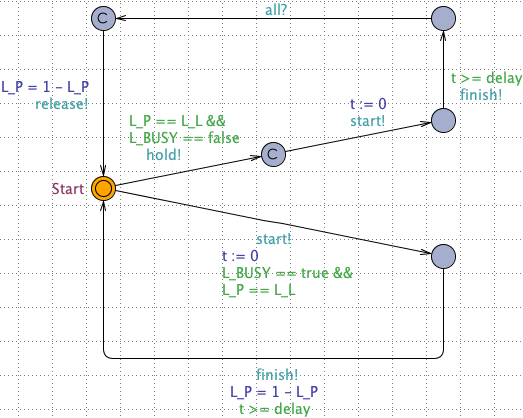
\includegraphics[width=10cm]{Person.png}
	\caption{\textbf{Person} - modelo.}
\end{figure}

Um aventureiro pode realizar uma travessia de 2 formas:
\begin{itemize}
	\item[-] \underline{com lanterna}: se a lanterna estiver livre e no mesmo local que o aventureiro, este pega na lanterna (\texttt{hold!}) e inicia imediatamente a travessia (\texttt{start!}).
	Neste ponto, pode esperar que outro aventureiro inicie também uma travessia, ou avança sozinho.
	
	Em ambos os casos, depois de esperar $delay$ minutos, diz ao processo \textbf{Bridge} que está pronto para acabar a travessia (\texttt{finish!}), e espera que este lhe responda indicando se todos os intervenientes da travessia já a acabaram (\texttt{all?}), podendo assim libertar a lanterna, atualizar a sua posição e voltar ao estado inicial, de modo a poder iniciar nova travessia (ou não).

	\item[-] \underline{sem lanterna}: o aventureiro só consegue iniciar a travessia se já existir um outro aventureiro que tenha iniciado a sua travessia com a lanterna e do mesmo lado que ele.
	Depois de iniciada a travessia, o sistema espera $delay$ minutos até poder acabar a sua travessia (\texttt{finish!}), voltando ao estado inicial com a sua posição atualizada.

	Apesar de ter voltado ao estado inicial, este aventureiro não pode iniciar outra travessia enquanto que a lanterna esteja liberta.
	O que acontece apenas quando o aventureiro com a lanterna acaba a sua travessia, e este só acaba quando todos os todos os que fizeram esta travessia acabarem. Isto pode ser visto como "acabar ao mesmo tempo", porque mesmo que um execute a ação \texttt{finish!} primeiro que o outro, a travessia só realmente acaba quando ambos estão do outro lado da ponte e a lanterna é largada, sendo o tempo da travessia igual ao maior $delay$ entre os intervenientes, como era pedido no exercício.
\end{itemize}




\section{Verificação}
\paragraph{Não existe \textit{deadlock}:}{
	$A \square\ \neg deadlock$
}

\begin{verbatim}
	A[] not deadlock
\end{verbatim}

\paragraph{É possível que todos os aventureiros estejam do outro lado da ponte em 17 minutos:}{
	$E \Diamond\ (\forall_{1 \leq i \leq 4}\ Person_{i}.L_P = 1) \land global = 17$
}

\begin{verbatim}
	E<> ((Person1.L_P == 1 and 
		  Person2.L_P == 1 and
		  Person3.L_P == 1 and
		  Person4.L_P == 1)
	and global == 17)
\end{verbatim}

\paragraph{É impossível que todos os aventureiros estejam no outro lado da ponte em menos de 17 minutos:}{
	$A \square\ \neg((\forall_{1 \leq i \leq 4}\ Person_{i}.L_P = 1) \land global < 17)$
}

\begin{verbatim}
	A[] not ((Person1.L_P == 1 and
			  Person2.L_P == 1 and
			  Person3.L_P == 1 and
			  Person4.L_P == 1)
	and global < 17)
\end{verbatim}


\section{Conclusão}
Após a demonstração da nossa abordagem a este problema, dá-se por concluído este trabalho prático.

De um modo geral estamos satisfeitos com o porque fizemos tudo o que foi pedido, e foi uma forma de conseguirmos aplicar os conteúdos que fomos aprendendo e assimilando ao longo desta UC, tanto na primeira parto do trabalho (modelação), como na segunda (verificação).

Numa nota final, podemos concluir que de facto a modelação é uma ferramenta forte porque nos permite investigar, testar ou até mesmo prever o comportamento de sistemas de vida real, sem que tenhamos de gastar recursos a construí-lo.
\end{document}
